\section{Results}\label{sec:results}
\mr{This section presents our $\fnl$ constraints from the DESI LRG targets. The analysis is not carried out blindly. However, the same codes are applied to the mocks to quantify biases associated with our methods. The contamination model used in the mock test is linear and assumed to be unknown and selected to be different from our default cleaning methods, which are nonlinear.} 


\subsection{DESI imaging LRG sample}
\begin{figure}
    \centering
    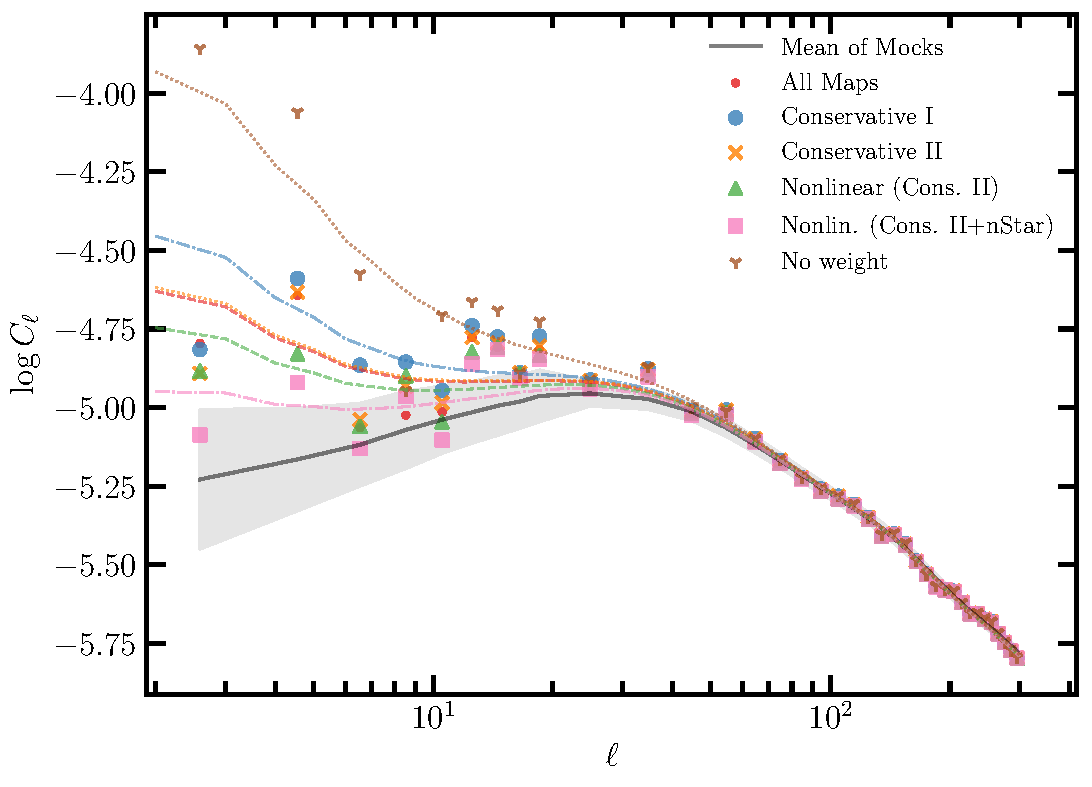
\includegraphics[width=0.45\textwidth]{figures/model_dr9.pdf} 
    \caption{The angular power spectrum of the DR9 LRG sample before (\textit{No weight}) and after correcting for imaging systematics using various methods with their corresponding best fit theory curves. The shade represents $1\sigma$ error constructed from the $\fnl=0$ mocks.}
    \label{fig:cl_dr9}
\end{figure}
Figure \ref{fig:cl_dr9} shows the measured power spectrum of the DR9 LRG sample before and after applying imaging weights and the best fit theory curves. The solid link and shade represent the mean power spectrum and 1$\sigma$ error estimated from the $\fnl=0$ lognormal simulations. The power spectra are similar on small scales ($\ell > 20$), but the differences between various cleaning methods are significant on large scales. By comparing \textit{linear conservative I} to \textit{linear conservative II}, we find that the measured clustering power on modes with $6\leq \ell < 10$ are noticeably different between the two methods. We associate the differences to the additional map for psfsize in the r-band for \textit{linear conservative II}. On other scales, the differences between the spectra after the linear-based cleaning are negligible, supporting the idea that our feature selection procedure has been effective to identify the primary maps causing the large-scale excess clustering signal. Comparing \textit{nonlinear conservative II} to \textit{linear conservative II}, we find that the measured spectra on $4 \leq \ell < 6$ are very different, probably indicating some nonlinear spurious fluctuations with large scale characteristics due to extinction. Including stellar density in the nonlinear approach (\textit{nonlinear conservative II + nStar}) further reduces the excess power relative to the mock power spectrum, in particular on modes between $2\leq \ell < 4$. We associate this to the flexibility of the nonlinear approach in correcting for systematics effects on multiples scales.

\subsubsection{Calibrated constraints}

\begin{figure}
    \raggedleft
    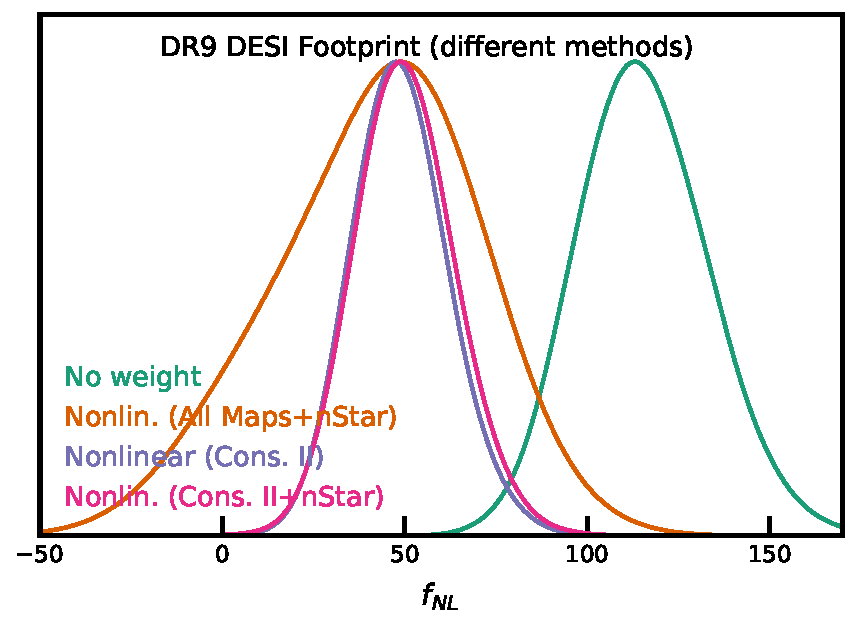
\includegraphics[width=0.424\textwidth]{mcmc_dr9methods1d.pdf}
    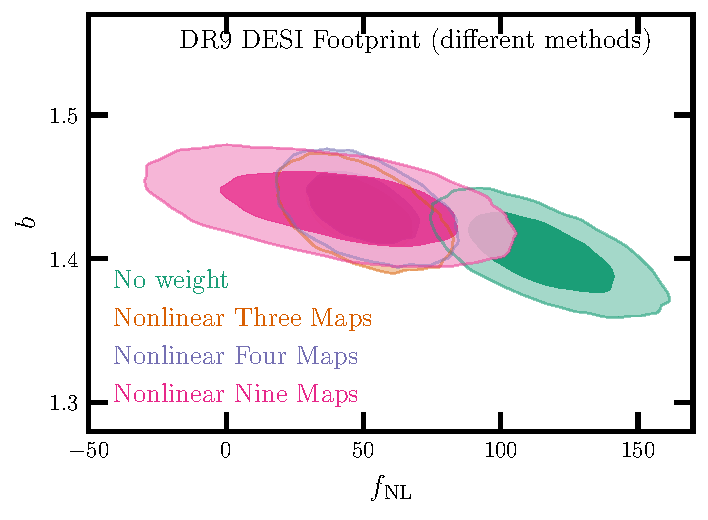
\includegraphics[width=0.45\textwidth]{figures/mcmc_dr9methods.pdf} 
    \caption{The calibrated constrains from the DR9 LRG targets. \textit{Top}: probability distribution for $\fnl$ marginalized over the shotnoise and bias. \textit{Bottom}: $68\%$ and $95\%$ probability distribution contours for the bias and $\fnl$ from the DR9 LRG sample before and after applying nonlinear cleaning methods. The lognormal mocks are used to calibrate these distributions for over correction.}\label{fig:mcmc_dr9}
\end{figure}

\begin{table*}
    \caption{The calibrated best fit and marginalized mean estimates for $\fnl$ from fitting power spectrum of the DESI DR9 LRG sample before and after correcting for systematics. Degree of freedom is 34 (37 data points - 3 parameters).}
    \label{tab:dr9methodcalib}
   \centerline{%     
    \begin{tabular}{llllllll}
    \hline
    \hline
   &  & 	  & & $\fnl$ &  &  \\
   \cmidrule(r{.7cm}){3-6}
Footprint                               & Method & 	Best fit  & Mean & $ 68\%$ CL & $ 95\%$ CL & $\chi^{2}$ \\
    \hline
DESI                      & No Weight   & $113.18$& $115.49$& $ 98.14<\fnl<132.89$& $ 83.51<\fnl<151.59$ &   44.4\\
DESI                      & Nonlinear (Cons. II)& $ 47.38$& $ 48.81$& $ 36.08<\fnl< 61.44$& $ 25.03<\fnl< 75.64$ &   34.6\\
DESI                      & Nonlinear (Cons. II+nStar)& $ 48.92$& $ 50.10$& $ 36.88<\fnl< 63.31$& $ 24.87<\fnl< 77.78$ &   35.2\\
DESI                      & Nonlinear (All Maps+nStar)& $ 49.69$& $ 41.91$& $ 13.10<\fnl< 69.14$& $-15.96<\fnl< 91.84$ &   39.5\\
   \hline
    \end{tabular}
}
\end{table*}

All $\fnl$ constraints presented here are calibrated for the effect of over correction using the lognormal simulations. Table \ref{tab:dr9methodcalib} describes the best fit and marginalized mean estimates of $\fnl$ from fitting the power spectrum of the DR9 LRG sample before and after cleaning with the nonlinear approach given various combinations of imaging systematic maps. Figure \ref{fig:mcmc_dr9} shows the marginalized probability distribution for $\fnl$ (top) and the $68\%$ and $95\%$ probability contours for the linear bias parameter and $\fnl$ (bottom) from our sample before (\textit{no weight}) and after applying various imaging weights. We obtain $36.08 (25.03) < \fnl < 61.44(75.64)$ with $\chi^{2}=34.6$ for \textit{nonlinear conservative II}, $36.88(24.87) < \fnl < 63.31(77.78)$ with $\chi^{2}=35.2$ for \textit{nonlinear conservative II + nStar}, and $13.10(-15.96) < \fnl < 69.14(91.84)$ with $\chi^{2}=39.5$ for \textit{nonlinear all maps + nStar} at $68\% (95\%)$ confidence over 34 degrees of freedom. Overall, we find the maximum likelihood estimates to be consistent among the various cleaning methods. For the conservative methods, the confidence intervals with or without $nStar$ are consistent with each other and more than $3\sigma$ off from zero PNG. The method \textit{nonlinear all maps+nStar} has asymmetric probability distribution with a larger uncertainty, and is consistent with $\fnl=0$ at $95\%$ confidence. For comparison, we obtain $98.14(83.51) < \fnl < 132.89(151.59)$ at $68\% (95\%)$ confidence with $\chi^{2}=44.4$ for the \textit{no weight} approach. The uncalibrated probability contours are presented in Appendix \ref{sec:dr9uncalib}.


\subsubsection{Uncalibrated constraints: robustness tests}
Now we proceed to perform some robustness tests and assess how sensitive the $\fnl$ constraints are to the assumptions made in the analysis or the quality cuts applied to the data. For each case, we re-train the cleaning methods and derive new sets of imaging weights. Accordingly, for the cases where a new survey mask is applied on the data, we re-calculate the covariance matrices using the new survey mask to account for the changes in the survey window and integral constraint effects. Calibrating the mitigation biases for all of these experiments is beyond the scope of this work and redundant. Therefore, the $\fnl$ constraints presented here are subject to the mitigation bias effect. Table \ref{tab:dr9method} describes the uncalibrated $\fnl$ constraints from the DR9 LRG sample. Our tests are as follows:

\begin{table*}
    \caption{The uncalibrated best fit and marginalized mean estimates for $\fnl$ from fitting power spectrum of the DR9 LRG sample before and after correcting for systematics. Degree of freedom is 34 (37 data points - 3 parameters). The lowest mode is $\ell=2$ and covariance matrix is from the $\fnl=0$ clean mocks (no mitigation) except for the case with '+cov' in which the covariance matrix is from the $\fnl=76.9$ clean mocks (no mitigation).}
    \label{tab:dr9method}
   \centerline{%     
    \begin{tabular}{llllllll}
    \hline
    \hline
   &  & 	  & & $\fnl$ &  &  \\
   \cmidrule(r{.7cm}){3-6}
Footprint                               & Method & 	Best fit  & Mean & $ 68\%$ CL & $ 95\%$ CL & $\chi^{2}$ \\
    \hline
DESI                                    & No Weight   & $113.18$& $115.49$& $ 98.14<\fnl<132.89$& $ 83.51<\fnl<151.59$ &   44.4\\
DESI                                    & Linear (All Maps)& $ 36.05$& $ 37.72$& $ 26.13<\fnl< 49.21$& $ 16.31<\fnl< 62.31$ &   41.1\\
DESI                                    & Linear (Conservative I)& $ 49.58$& $ 51.30$& $ 38.21<\fnl< 64.33$& $ 27.41<\fnl< 78.91$ &   38.8\\
DESI                                    & Linear (Conservative II)& $ 36.63$& $ 38.11$& $ 26.32<\fnl< 49.86$& $ 16.36<\fnl< 63.12$ &   39.6\\
DESI                                    & Nonlinear (Cons. II)& $ 28.58$& $ 29.79$& $ 18.91<\fnl< 40.59$& $  9.47<\fnl< 52.73$ &   34.6\\
DESI                                    & Nonlin. (Cons. II+nStar)& $ 16.63$& $ 17.52$& $  7.51<\fnl< 27.53$& $ -1.59<\fnl< 38.49$ &   35.2\\
DESI                                    & Nonlin. (All Maps+nStar)& $ -5.87$& $ -9.19$& $-21.45<\fnl<  2.40$& $-33.81<\fnl< 12.06$ &   39.5\\
DESI (imag. cut)                  & Nonlin. (Cons. II)& $ 29.16$& $ 30.57$& $ 19.05<\fnl< 42.18$& $  9.01<\fnl< 54.81$ &   35.8\\
DESI (comp. cut)                 & Nonlin. (Cons. II)& $ 28.07$& $ 29.48$& $ 18.38<\fnl< 40.50$& $  8.81<\fnl< 53.10$ &   34.5\\
DESI                                    & Nonlin. (Cons. II) + cov& $ 31.62$& $ 33.11$& $ 20.94<\fnl< 45.24$& $ 10.56<\fnl< 59.16$ &   33.5\\
\hline
BASS+MzLS                        & Nonlin. (Cons. II)& $ 15.43$& $ 19.01$& $ -1.17<\fnl< 39.43$& $-19.19<\fnl< 63.56$ &   35.6\\
BASS+MzLS                        & Nonlin. (Cons. II+nStar)& $ 13.12$& $ 15.39$& $ -4.59<\fnl< 35.56$& $-24.88<\fnl< 59.31$ &   34.7\\
BASS+MzLS                        & Nonlin. (All Maps+nStar)& $ -3.73$& $ -6.34$& $-27.11<\fnl< 13.75$& $-47.44<\fnl< 33.94$ &   36.8\\
BASS+MzLS (imag. cut)      & Nonlin. (Cons. II)& $ 25.03$& $ 29.12$& $  6.16<\fnl< 52.44$& $-14.22<\fnl< 80.54$ &   36.2\\
BASS+MzLS (comp. cut)     & Nonlin. (Cons. II)& $ 16.99$& $ 20.90$& $  0.26<\fnl< 41.76$& $-18.30<\fnl< 67.12$ &   35.8\\
DECaLS North                     & Nonlin. (Cons. II)& $ 41.02$& $ 44.89$& $ 23.33<\fnl< 66.78$& $  4.96<\fnl< 93.02$ &   41.1\\
DECaLS North                     & Nonlin. (Cons. II+CALIBZ+HI)& $ 55.46$& $ 60.44$& $ 36.78<\fnl< 84.05$& $ 17.86<\fnl<112.81$ &   38.4\\
DECaLS North                     & Nonlin. (Cons. II+nStar)& $ 31.45$& $ 34.78$& $ 14.14<\fnl< 55.79$& $ -5.81<\fnl< 80.80$ &   41.2\\
DECaLS North                     & Nonlin. (All Maps+nStar)& $  0.81$& $ -5.68$& $-29.73<\fnl< 16.71$& $-53.15<\fnl< 36.19$ &   45.1\\
DECaLS North (no DEC cut)      & Nonlin. (Cons. II)& $ 41.05$& $ 44.82$& $ 23.58<\fnl< 66.08$& $  6.40<\fnl< 91.42$ &   40.7\\
DECaLS North (imag. cut)   & Nonlin. (Cons. II)& $ 43.27$& $ 48.39$& $ 24.60<\fnl< 72.50$& $  4.71<\fnl<101.42$ &   35.1\\
DECaLS North (comp. cut)  & Nonlin. (Cons. II)& $ 40.55$& $ 44.63$& $ 22.41<\fnl< 67.11$& $  3.95<\fnl< 94.06$ &   41.4\\
DECaLS South                    & Nonlin. (Cons. II)& $ 31.24$& $ 33.21$& $ 14.89<\fnl< 52.40$& $ -5.11<\fnl< 74.35$ &   30.2\\
DECaLS South                    & Nonlin. (Cons. II+CALIBZ+HI)& $ 33.79$& $ 37.50$& $ 17.71<\fnl< 57.42$& $ -0.31<\fnl< 80.94$ &   30.8\\
DECaLS South                    & Nonlin. (Cons. II+nStar)& $ 14.34$& $  6.28$& $-21.19<\fnl< 30.01$& $-53.63<\fnl< 49.51$ &   31.9\\
DECaLS South                    & Nonlin. (All Maps+nStar)& $-36.76$& $-32.01$& $-49.38<\fnl<-13.61$& $-65.26<\fnl<  7.52$ &   31.5\\
DECaLS South (no DEC cut) & Nonlin. (Cons. II)& $ 43.79$& $ 46.79$& $ 30.16<\fnl< 63.41$& $ 16.38<\fnl< 82.72$ &   23.8\\
DECaLS South (imag. cut)        & Nonlin. (Cons. II)& $ 26.47$& $ 23.36$& $  3.18<\fnl< 47.84$& $-57.69<\fnl< 71.39$ &   30.0\\
DECaLS South (comp. cut)       & Nonlin. (Cons. II)& $ 29.62$& $ 31.76$& $ 13.00<\fnl< 51.58$& $ -9.78<\fnl< 74.28$ &   29.7\\
   \hline
    \end{tabular}}
\end{table*}

\begin{figure}
    \centering
    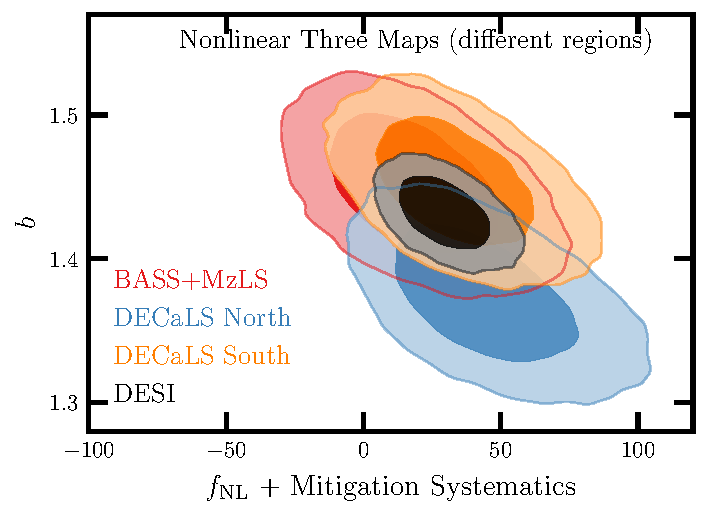
\includegraphics[width=0.45\textwidth]{figures/mcmc_dr9regions.pdf} 
    \caption{The uncalibrated 2D constraints from the DR9 LRG sample for each imaging survey compared with that for the whole DESI footprint. The dark and light shades represent the $68\%$ and $95\%$ confidence intervals, respectively.}\label{fig:mcmc_dr9reg}
\end{figure}
\begin{figure}
    \centering
    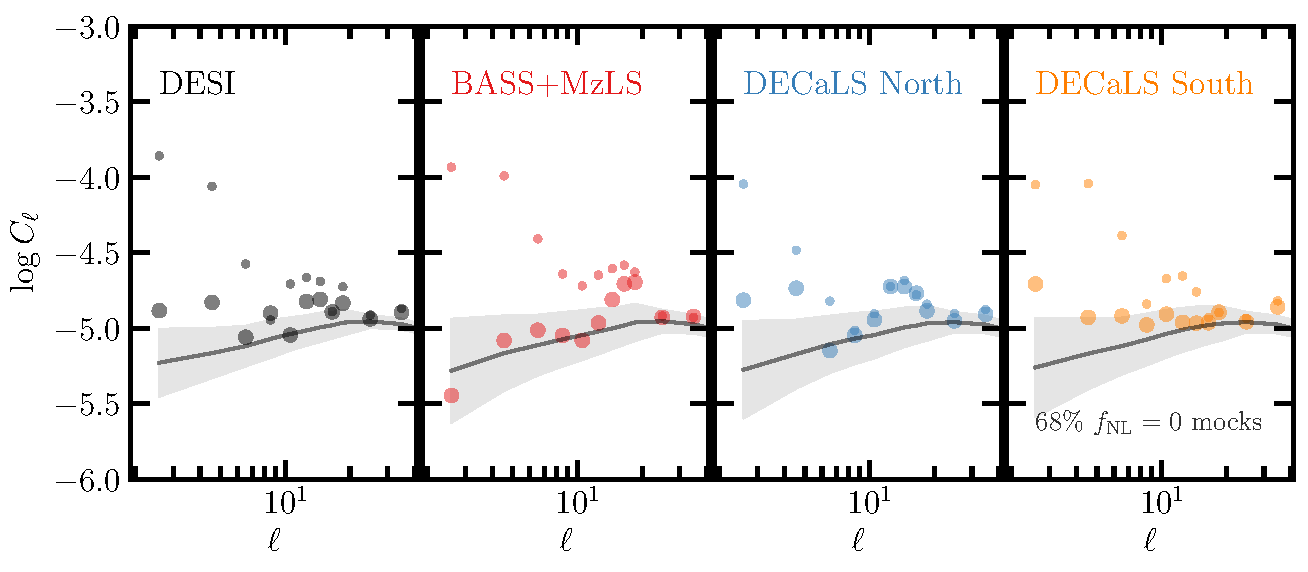
\includegraphics[width=0.45\textwidth]{figures/cldr9_lowell.pdf}
    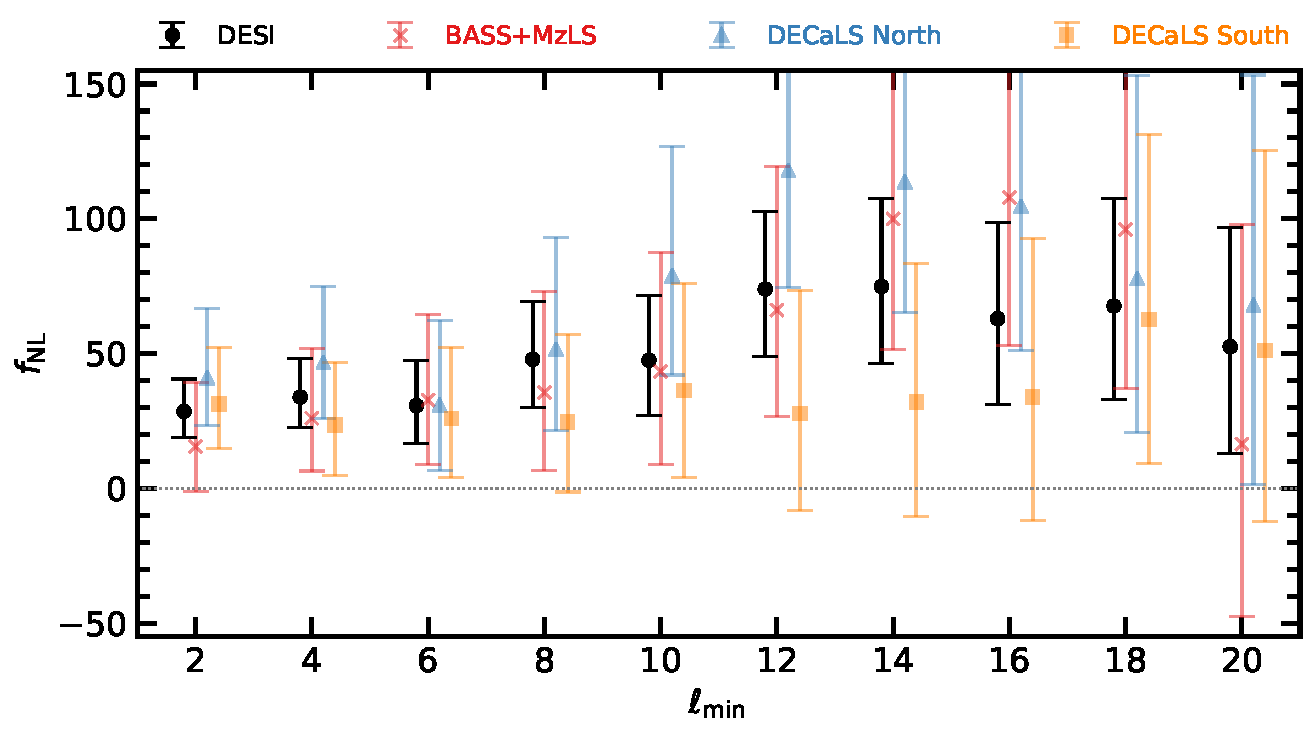
\includegraphics[width=0.46\textwidth]{figures/fnl_elmin.pdf}  
    \caption{Top: The measured power spectra before and after \textit{nonlinear conservative II}. The uncalibrated $\fnl$ constraints vs the lowest $\ell$ mode from with the DR9 LRG sample cleaned with \textit{nonlinear conservative II}. The points represent marginalized mean estimates of $\fnl$ and errorbars represent $68$\% confidence.}\label{fig:mcmc_dr9elmin}
\end{figure}

\begin{itemize}[itemindent=*]

\item \textbf{Linear methods}: We find consistent $\fnl$ constraints from \textit{linear all maps} and \textit{linear conservative II} which suggests that \bbk{not} all imaging systematic maps are \bbk{\sout{not}} needed to completely mitigate systematic effects. We find $\sigma (\fnl) \sim 25$ for the linear methods. With the same set of imaging systematic maps, the nonlinear method yields smaller constraint, $\Delta \fnl = -8$, and a better $\chi^{2}$ fit, e.g., $34.6$ vs $39.6$.

\item \textbf{Imaging regions}: We compare how the $\fnl$ constraints from fitting the power spectrum of the whole DESI footprint compares to that from the power spectrum for each imaging region individually, namely BASS+MzLS, DECaLS North, and DECaLS South. Figure \ref{fig:mcmc_dr9reg} shows the $68\%$ and $95\%$ probability contours on $\fnl$ and $b$ from each individual region, compared with that from DESI. The cleaning method here is \textit{nonlinear conservative II}. Overall, we find that the constraints from all imaging surveys are consistent with each other within $68\%$ confidence. Both BASS+MzLS and DECaLS South yield constraints consistent with $\fnl=0$ within $95\%$, but DECaLS North deviates from zero PNG at more than $2\sigma$. This motivates follow-up studies with the spectroscopic sample of LRGs in DECaLS North.

\item \textbf{Stellar density template (\textit{nStar})}: Adding the stellar density template (\textit{nonlinear conservative II+ nStar}) does not change the constraints from BASS+MzLS much, but it shifts the $\fnl$ distributions to lower values in DECaLS North and DECaLS South by $0.5\sigma$ and $\sigma$, respectively, reconciling all constraints with $\fnl=0$. We note that differences are more significant when all maps and stellar density are used as input. This is somewhat expected as cleaning the data with more imaging systematic maps is more prone to the over-correction issue. \mr{We find that the shifts in $\fnl$ from adding $nStar$ are cancelled after accounting for the over correction bias. Comparing \textit{nonlinear conservative II+nStar} and \textit{nonlinear conservative II} in Table \ref{tab:dr9methodcalib} and \ref{tab:dr9method} is indicative that the $\fnl$ shifts are signs of over-correction due to correlations between the stellar density template and large-scale structure.} 

\item \textbf{Pixel completeness (\textit{comp. cut})}: We discard pixels with fractional completeness less than half to assess the effect of partially complete pixels on $\fnl$. This cut removes $0.6\%$ of the survey area, and no changes in the $\fnl$ constraints are observed.

\item \textbf{Imaging quality (\textit{imag. cut})}: Pixels with poor photometry are removed from our sample by applying the following cuts on imaging; $E[B-V]<0.1$, $nStar < 3000$, ${\rm depth}_{g} > 23.2$, ${\rm depth}_{r} > 22.6$, ${\rm depth}_{z} > 22.5$, ${\rm psfsize}_{g}<2.5$, ${\rm psfsize}_{r}<2.5$, and ${\rm psfsize}_{z}<2$. Despite losing $8\%$ of the survey mask, we obtain a negligible effect on the best fit $\fnl$ estimate from fitting the DESI power spectrum. When each region is fit separately, we find that the BASS+MzLS constraint increases by $\Delta \fnl \sim 10$ while the constraints from DECaLS North and DECaLS South do not show significant changes. 

\item \textbf{Covariance matrix (\textit{cov})}: We fit the same LRG power spectrum with \textit{nonlinear conservative II} correction, but use a covariance matrix constructed from the $\fnl=76.92$ mocks. With the new covariance, a $12\%$ increase in the $\sigma \fnl$ is observed. We also find that the best fit and marginalized mean estimates of $\fnl$ increase by $10-11\%$. Overall, we find that the differences are not significant in comparison to the statistical precision.

\item \textbf{External maps (\textit{CALIBZ+HI})}: The nonlinear \textit{conservative II} method is re-trained with two additional external maps for the neutral hydrogen column density (HI) and the z-band photometric calibration error (CALIBZ). This test is only performed for the DECaLS region due to the data availability limitations and issues with the maps. With this correction, we find that the best fit $\fnl$ increases from $41.02$ to $55.46$ for DECaLS North and from $31.24$ to $33.79$ for DECaLS South. This might suggest that adding these two maps increases the input noise and thus negatively impacts the performance of the model.

\item \textbf{Declination mask (\textit{no DEC cut})}: The fiducial mask removes the spurious disconnected islands in DECaLS North and regions with DEC $<-30$ in DECaLS South, where there is a high likelihood of calibration issues as different standard stars are used for photometric calibrations. We analyze our sample without these cuts, and find that the best fit and marginalized $\fnl$ mean estimates from DECaLS South shift significantly by $\Delta \fnl \sim 10$ which supports the issue of photometric systematics in the DECaLS South region below DEC $=-30$. While the constraints from DECaLS North do not change significantly. \bbk{[Did you try cutting out more of DECaLS North, such as everything below the equator?]}

\item \textbf{Scale dependence (\textit{varying $\ell_{\rm min}$})}: This test decreases the largest scale (or increase the lowest harmonic mode $\ell_{\rm min}$) while fitting the power spectrum. Figure \ref{fig:mcmc_dr9elmin} illustrates the power spectra before and after \textit{nonlinear conservative II} in the top panel. The bottom panel shows the marginalized mean and $68\%$ error on $\fnl$ with \textit{nonlinear conservative II} for the DESI, BASS+MzLS, DECaLS North, and DECaLS South regions. \mr{ALEX: We find that the mean estimates of $\fnl$ slightly shifts to higher values on scales $12<\ell<18$ in DECaLS North and BASS+MzLS when higher $\ell_{\rm min}$ is used. This is the opposite behavior from what one would expect if there were just a giant systematics induced spike at low ell. So it shows that the issue here is more subtle than what one would have initially suspected.}

\end{itemize}

\subsection{Summary}
In summary, we find that the nonlinear methods outperform the linear methods in removing the excess clustering signal on large scales. Adding the stellar density map results in significant changes, however when accounted for the mitigation bias, all methods recover the same maximum likelihood estimate. With calibration on the lognormal mocks, the conservative approaches that use a small subset of imaging systematic maps show $\fnl$ detection at more than $2\sigma$ confidence. The most flexible nonlinear method with all maps and stellar density returns a bigger associated uncertainty which is consistent with $\fnl=0$. We also run various tests with cuts on the DR9 sample or changing the configuration or details of the analysis. Overall, we find consistent results across sub imaging surveys within DESI. However, our results show that a declination cut at DEC $=-30$ is necessary for DECaLS South to avoid potential calibration issues. Our analysis does not show a statistical demand for including external templates for HI and CALIBZ, using a different covariance matrix, or imposing additional cuts on the DR9 based on imaging and pixel completeness. We also obtain robust results regardless of the largest scale used for constraining $\fnl$.